\chapter{シス研というサークルについて}

\section{はじめに}
初めまして!シス研会長の林です!
はい、ここでみなさんシス研とはなんぞ?となっていると思うのでまずは自分が水先案内人となりましてシス研とこの本について解説していこうと思います。

\subsection{どんな話をするのか}
シス研ってどんなサークル?どんな活動をしているの?この本はどういったもの?といったものを紹介していきます。それでは、さっそく行ってみましょう!!!

\section{シス研とは}
シス研は正式名称を「システム工学研究会」と言い、愛知工業大学公認の情報系サークルです。歴史は長く、2023年で創立47周年を迎え、かのAppleと同い年となります!! \\
シス研ではハッカソン出場をはじめとしたチーム開発、ゲーム作成、インフラの構築、運用などを行っています。

\subsection{どんな活動をしているの?}
シス研の主な活動はチーム開発とインフラ整備です。サークル全体としての開発物などはなく、それぞれがチームを組んでハッカソンに出場したりしています。 \\
インフラ面では、部室に物理サーバを持っており、そこでシス研のホームページ\footnote{シス研ホームページ\url{https://set1.ie.aitech.ac.jp}}や各種サービス\footnote{シス研紹介ページ\url{https://welcome.sysken.net}}を公開しています。23年4月現在、大幅な工事を行なっておりごく一部のサービスのみ稼働しています(すみません)。
そのほかにもシス研主催のLT会・ハッカソンの開催、STECH様\footnote{STECH様HP \url{https://stech.careerselect.jp}}と共同でQiita Advent Calendar 2022\footnote{Qiita Advent Calendar 2022 \url{https://qiita.com/advent-calendar/2022/stech-ait-advent}}への参加もしています。
\begin{figure}[bht]
  \centering
  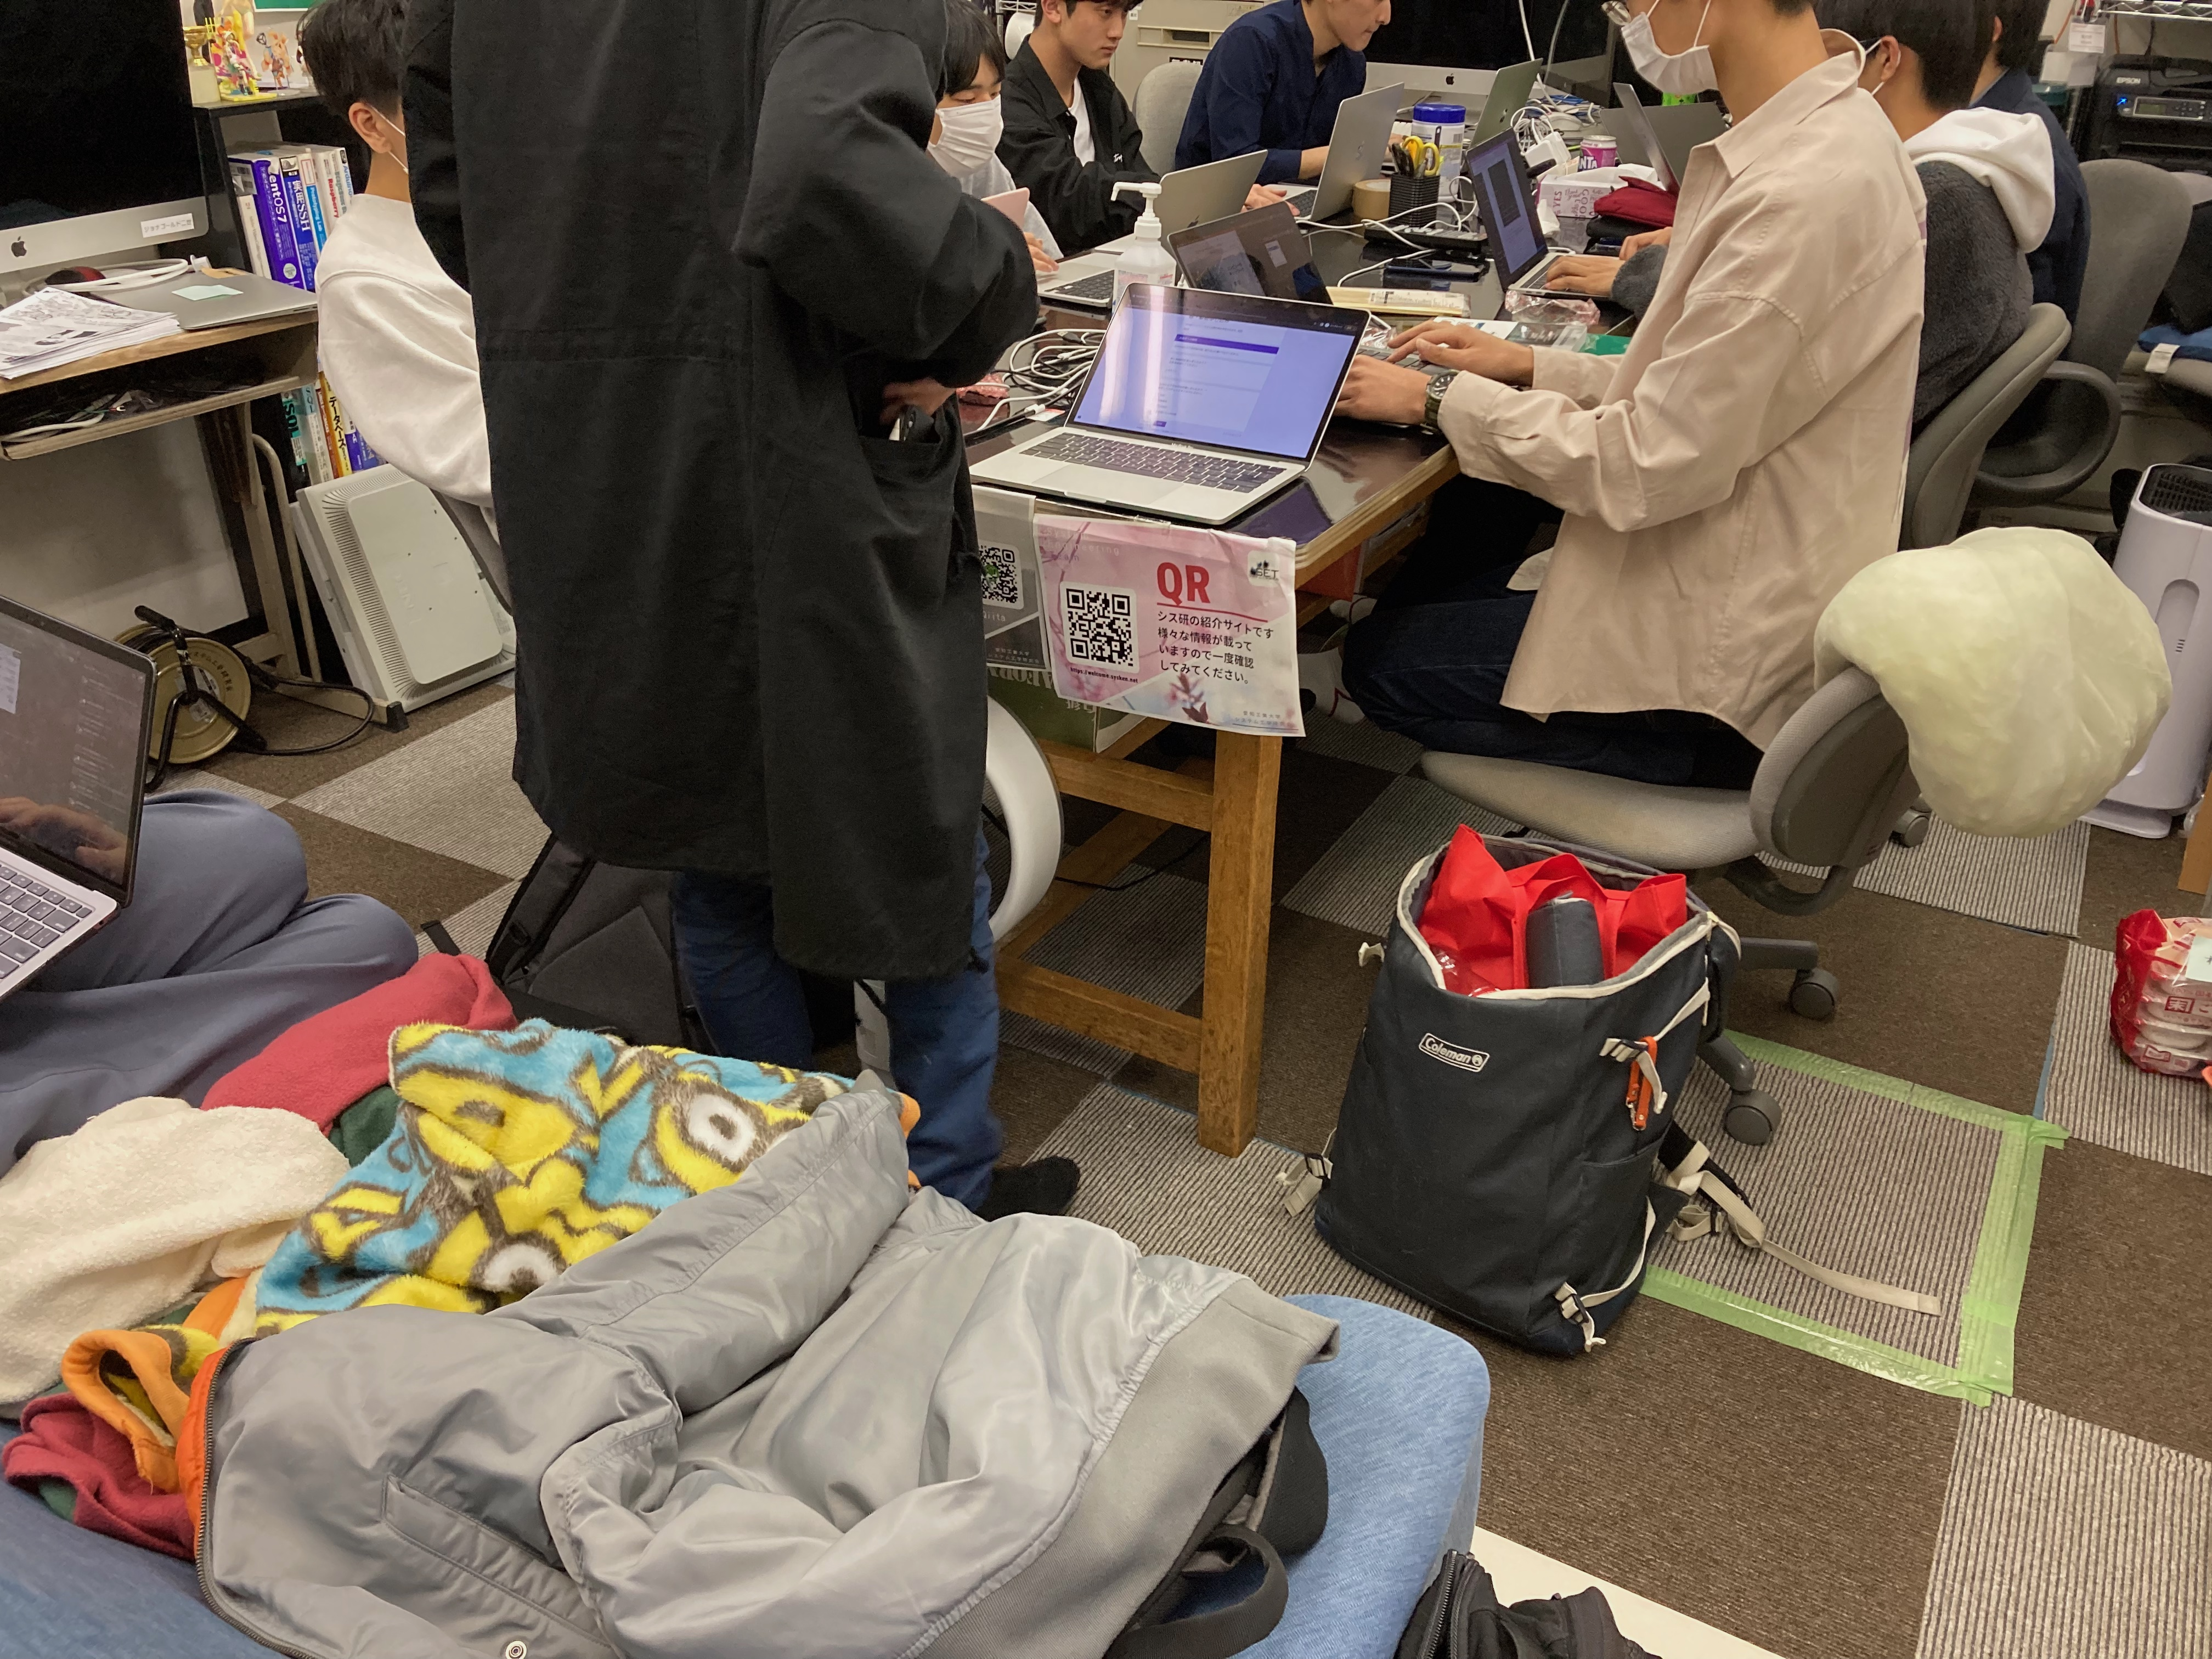
\includegraphics[width=10cm]{./image/02-AboutSysken/room.jpg}
  \caption{部室の様子}
\end{figure}

\subsection{2021〜2022年度の活動実績}
\begin{itemize}
  \item 2021 愛工大大学祭 工科展 最優秀賞
  \item 2022 技育CAMP vol3 努力賞
  \item 2022 技育CAMP vol4 努力賞
  \item 2022 技育博 参加
  \item 2022 技育CAMP vol8 優秀賞
  \item 2022 技育CAMP vol9 努力賞
  \item 2022 愛工大大学祭 工科展 瑞若賞
  \item 2022 技育展 出展
  \item 2022 愛工大大学祭 模擬店 最優秀賞
  \item 2022 Open Hack U 2022 ONLINE 参加
  \item 2022 技育CAMPアドバンス 登壇
  \item 2023 Open Hack U 2022 Spring ONLINE 参加
  \item 長期休暇中のLT会、ハッカソン主催
  \item 各種勉強会の開催
\end{itemize}

\begin{tcolorbox}[title=シス研の設備]
  \begin{itemize}
    \item ラックマウントサーバ、ネットワーク機器
    \item デスクトップPC
    \item iMac,MacBook
    \item iPhone,iPad
    \item Android端末各種
    \item Raspberry Pi
    \item はんだ等の電子工作セット
    \item その他多数...
  \end{itemize} 
\end{tcolorbox}

\begin{figure}[H]
  \begin{tabular}{cc}
    \begin{minipage}[b]{0.40\columnwidth}
      \centering
      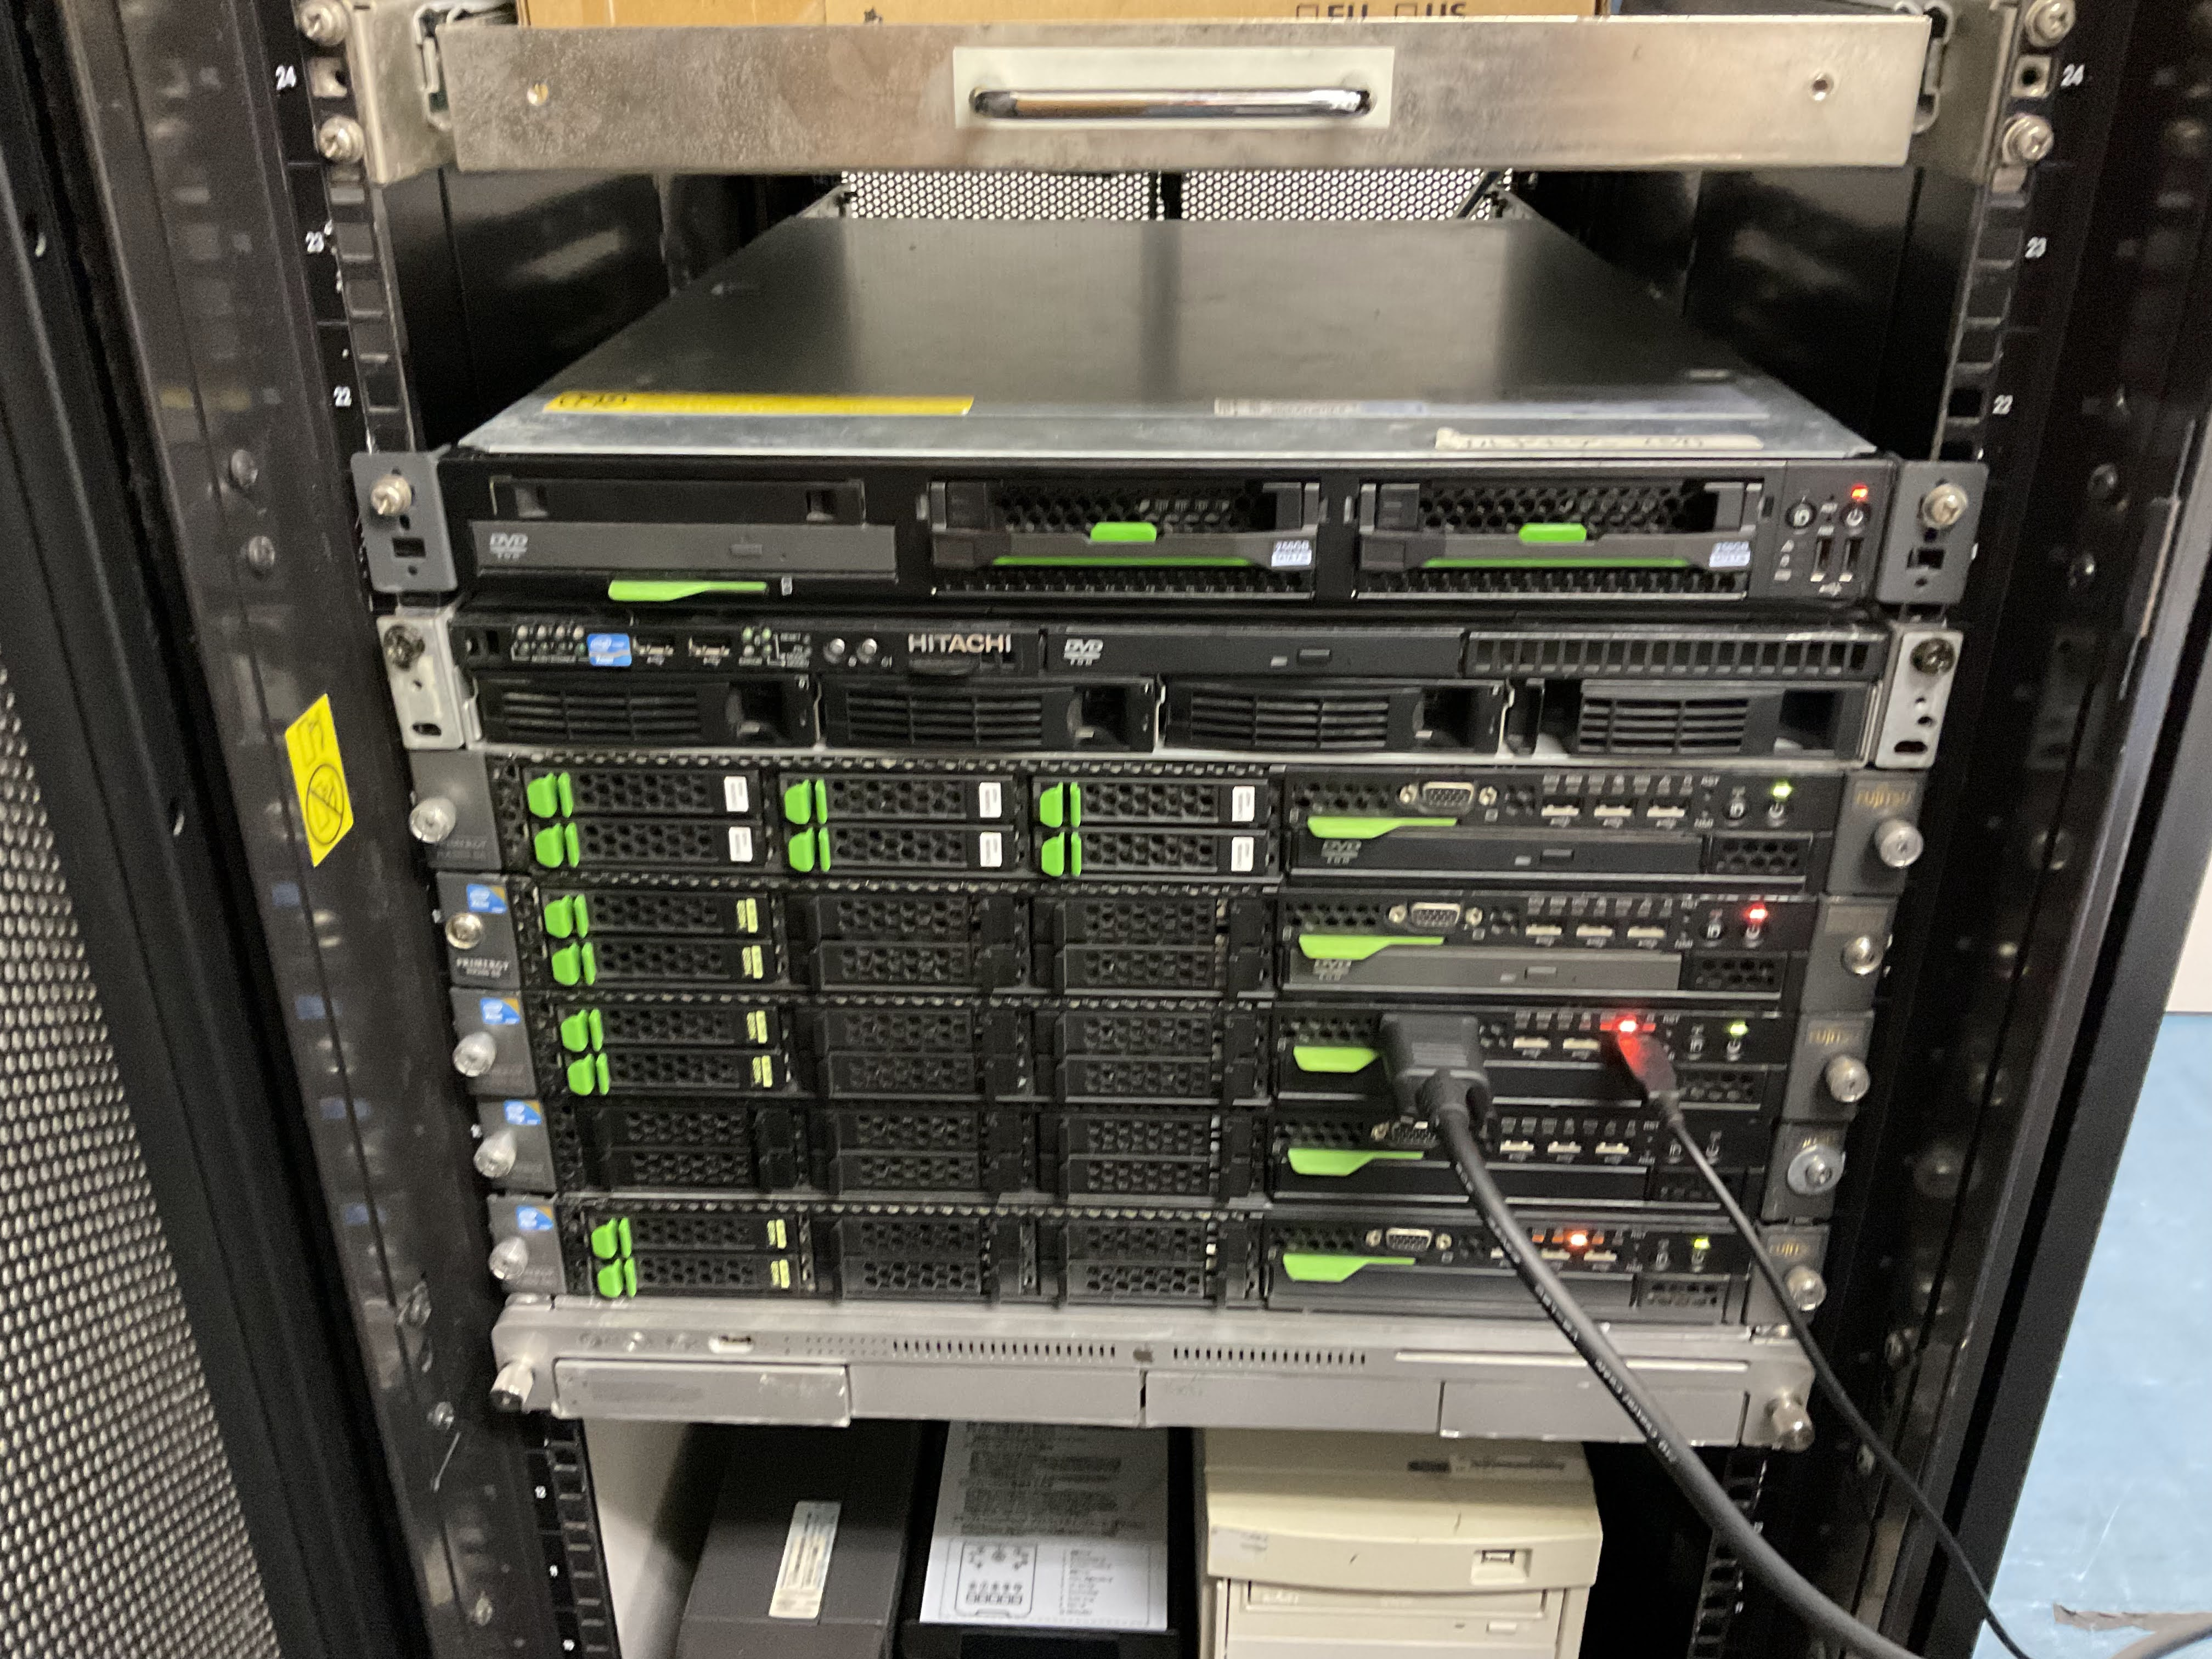
\includegraphics[width=\columnwidth]{./image/02-AboutSysken/server.jpg}
      \caption{ラックマウントサーバ}
    \end{minipage} &
    \hspace{0.04\columnwidth}
    \begin{minipage}[b]{0.40\columnwidth}
      \centering
      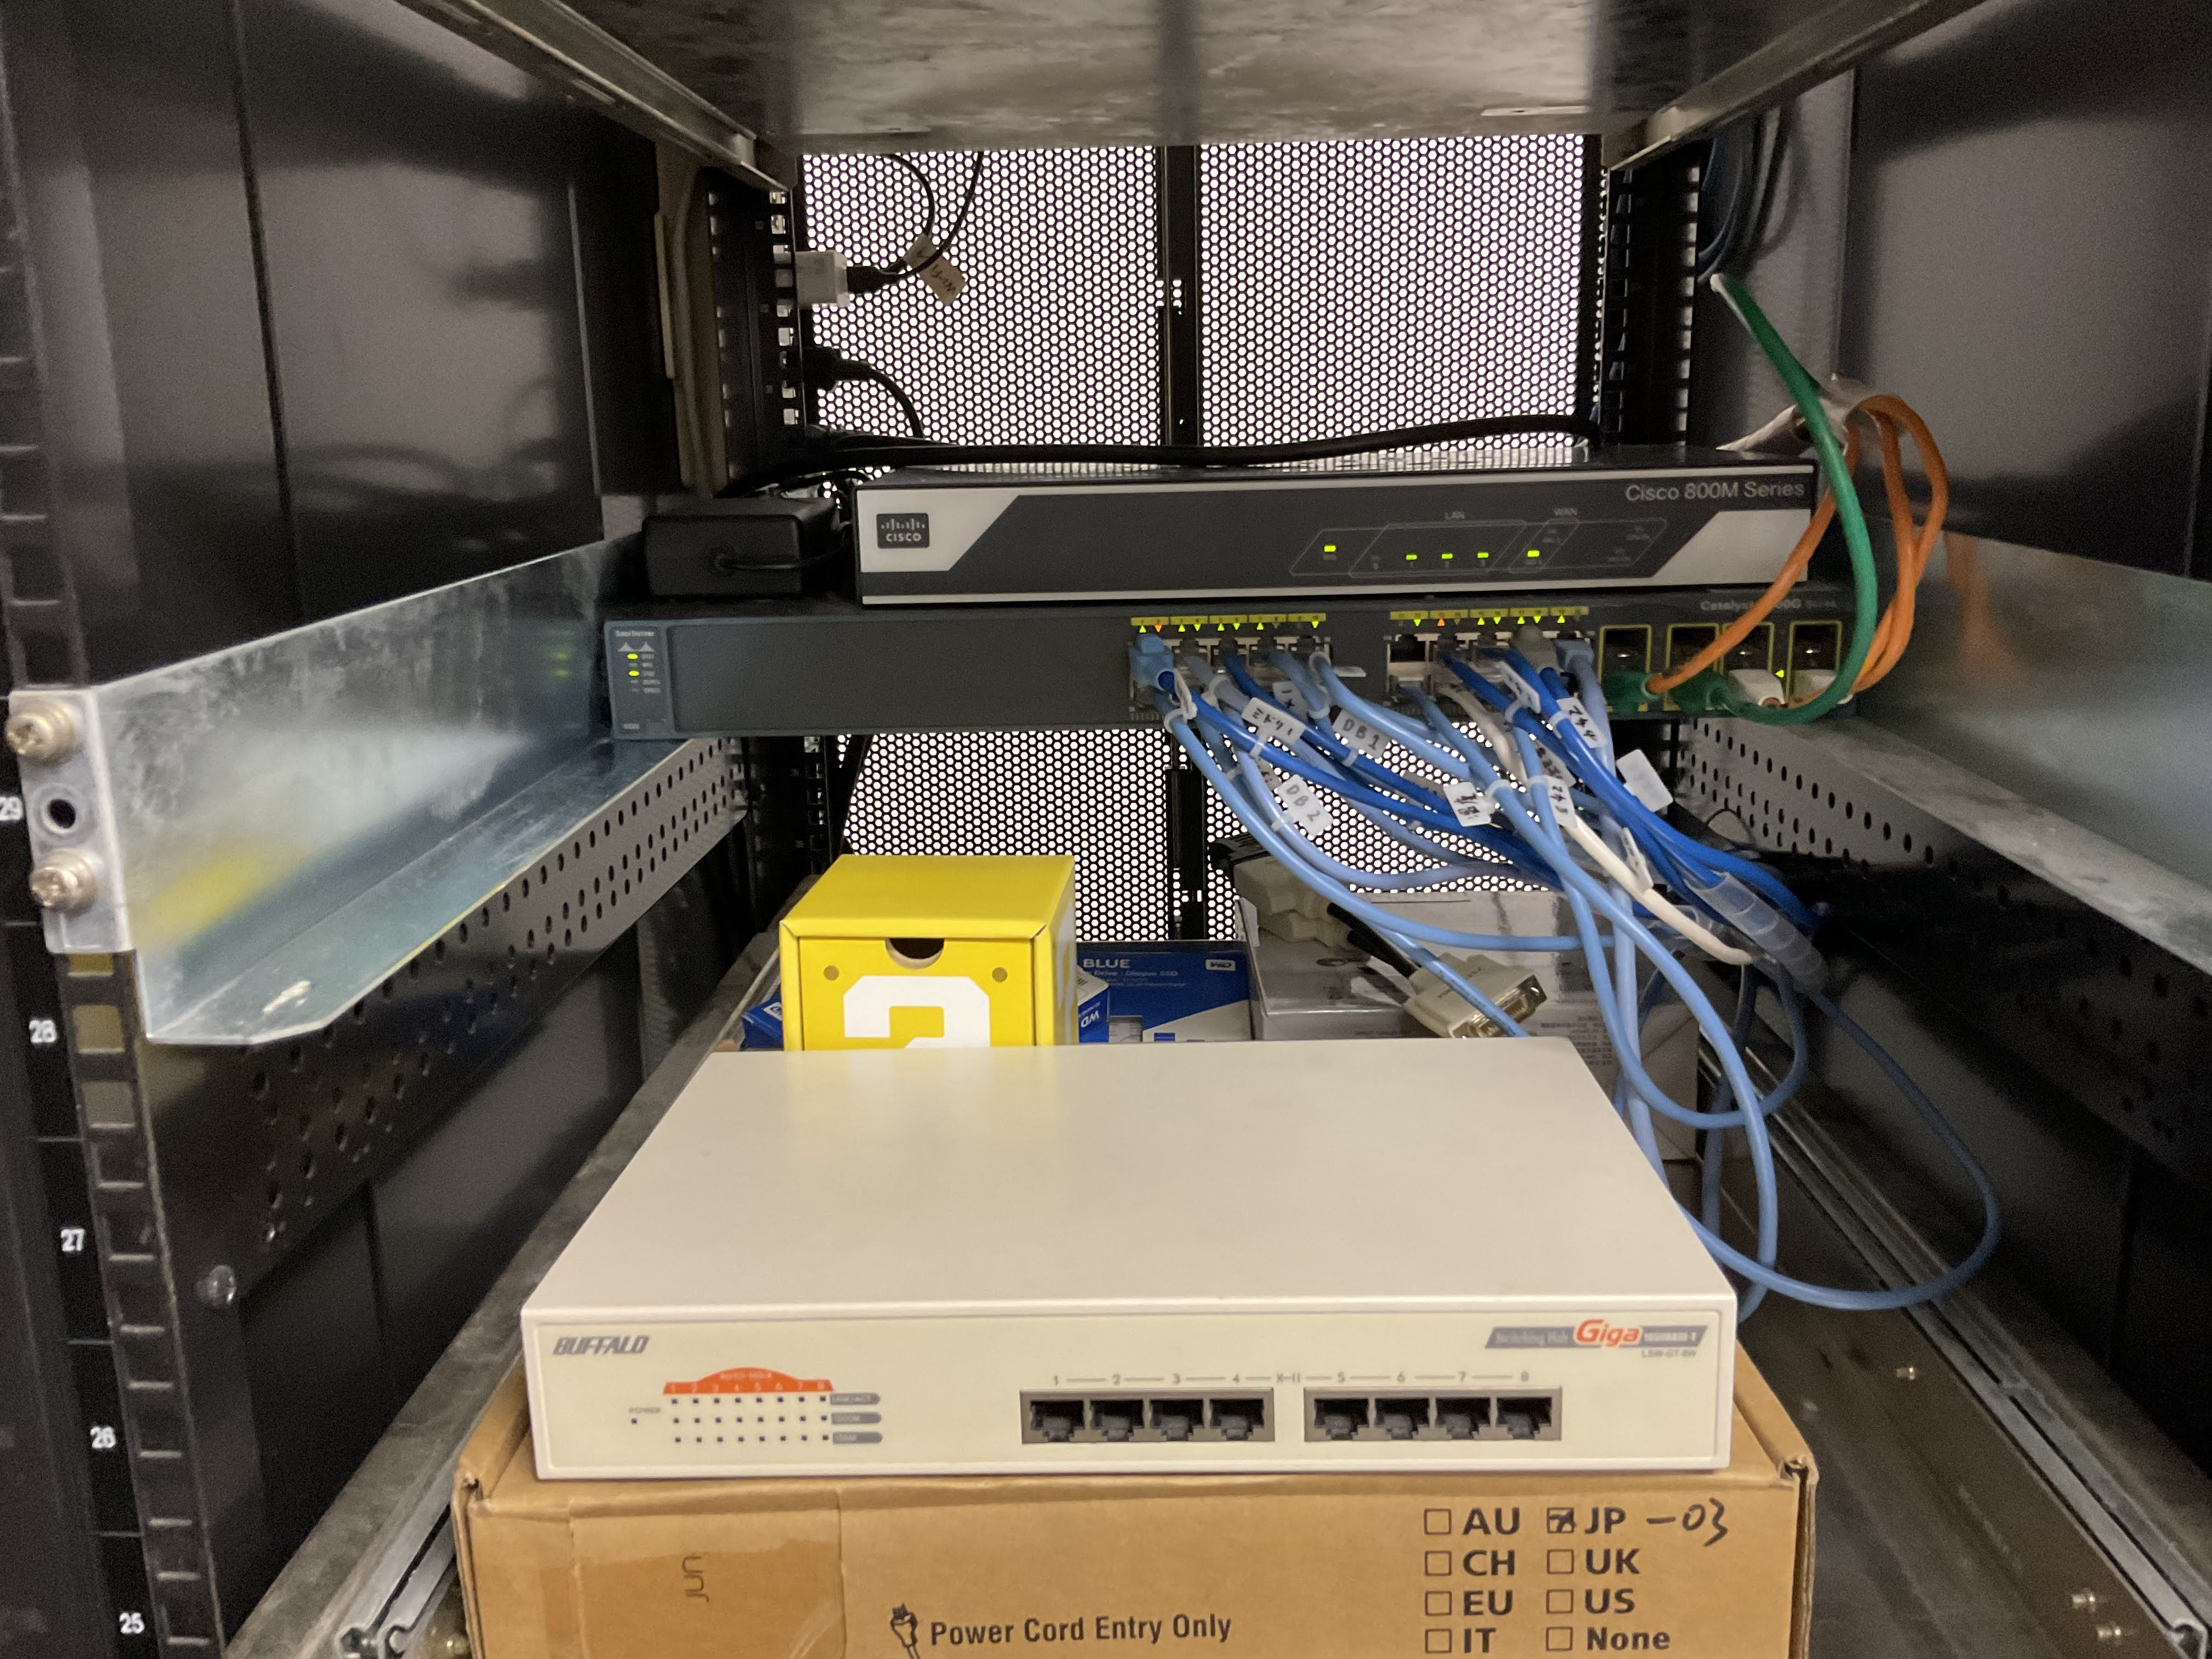
\includegraphics[width=\columnwidth]{./image/02-AboutSysken/network.jpg}
      \caption{ネットワーク機器}
    \end{minipage} \\
    \begin{minipage}[b]{0.40\columnwidth}
      \centering
      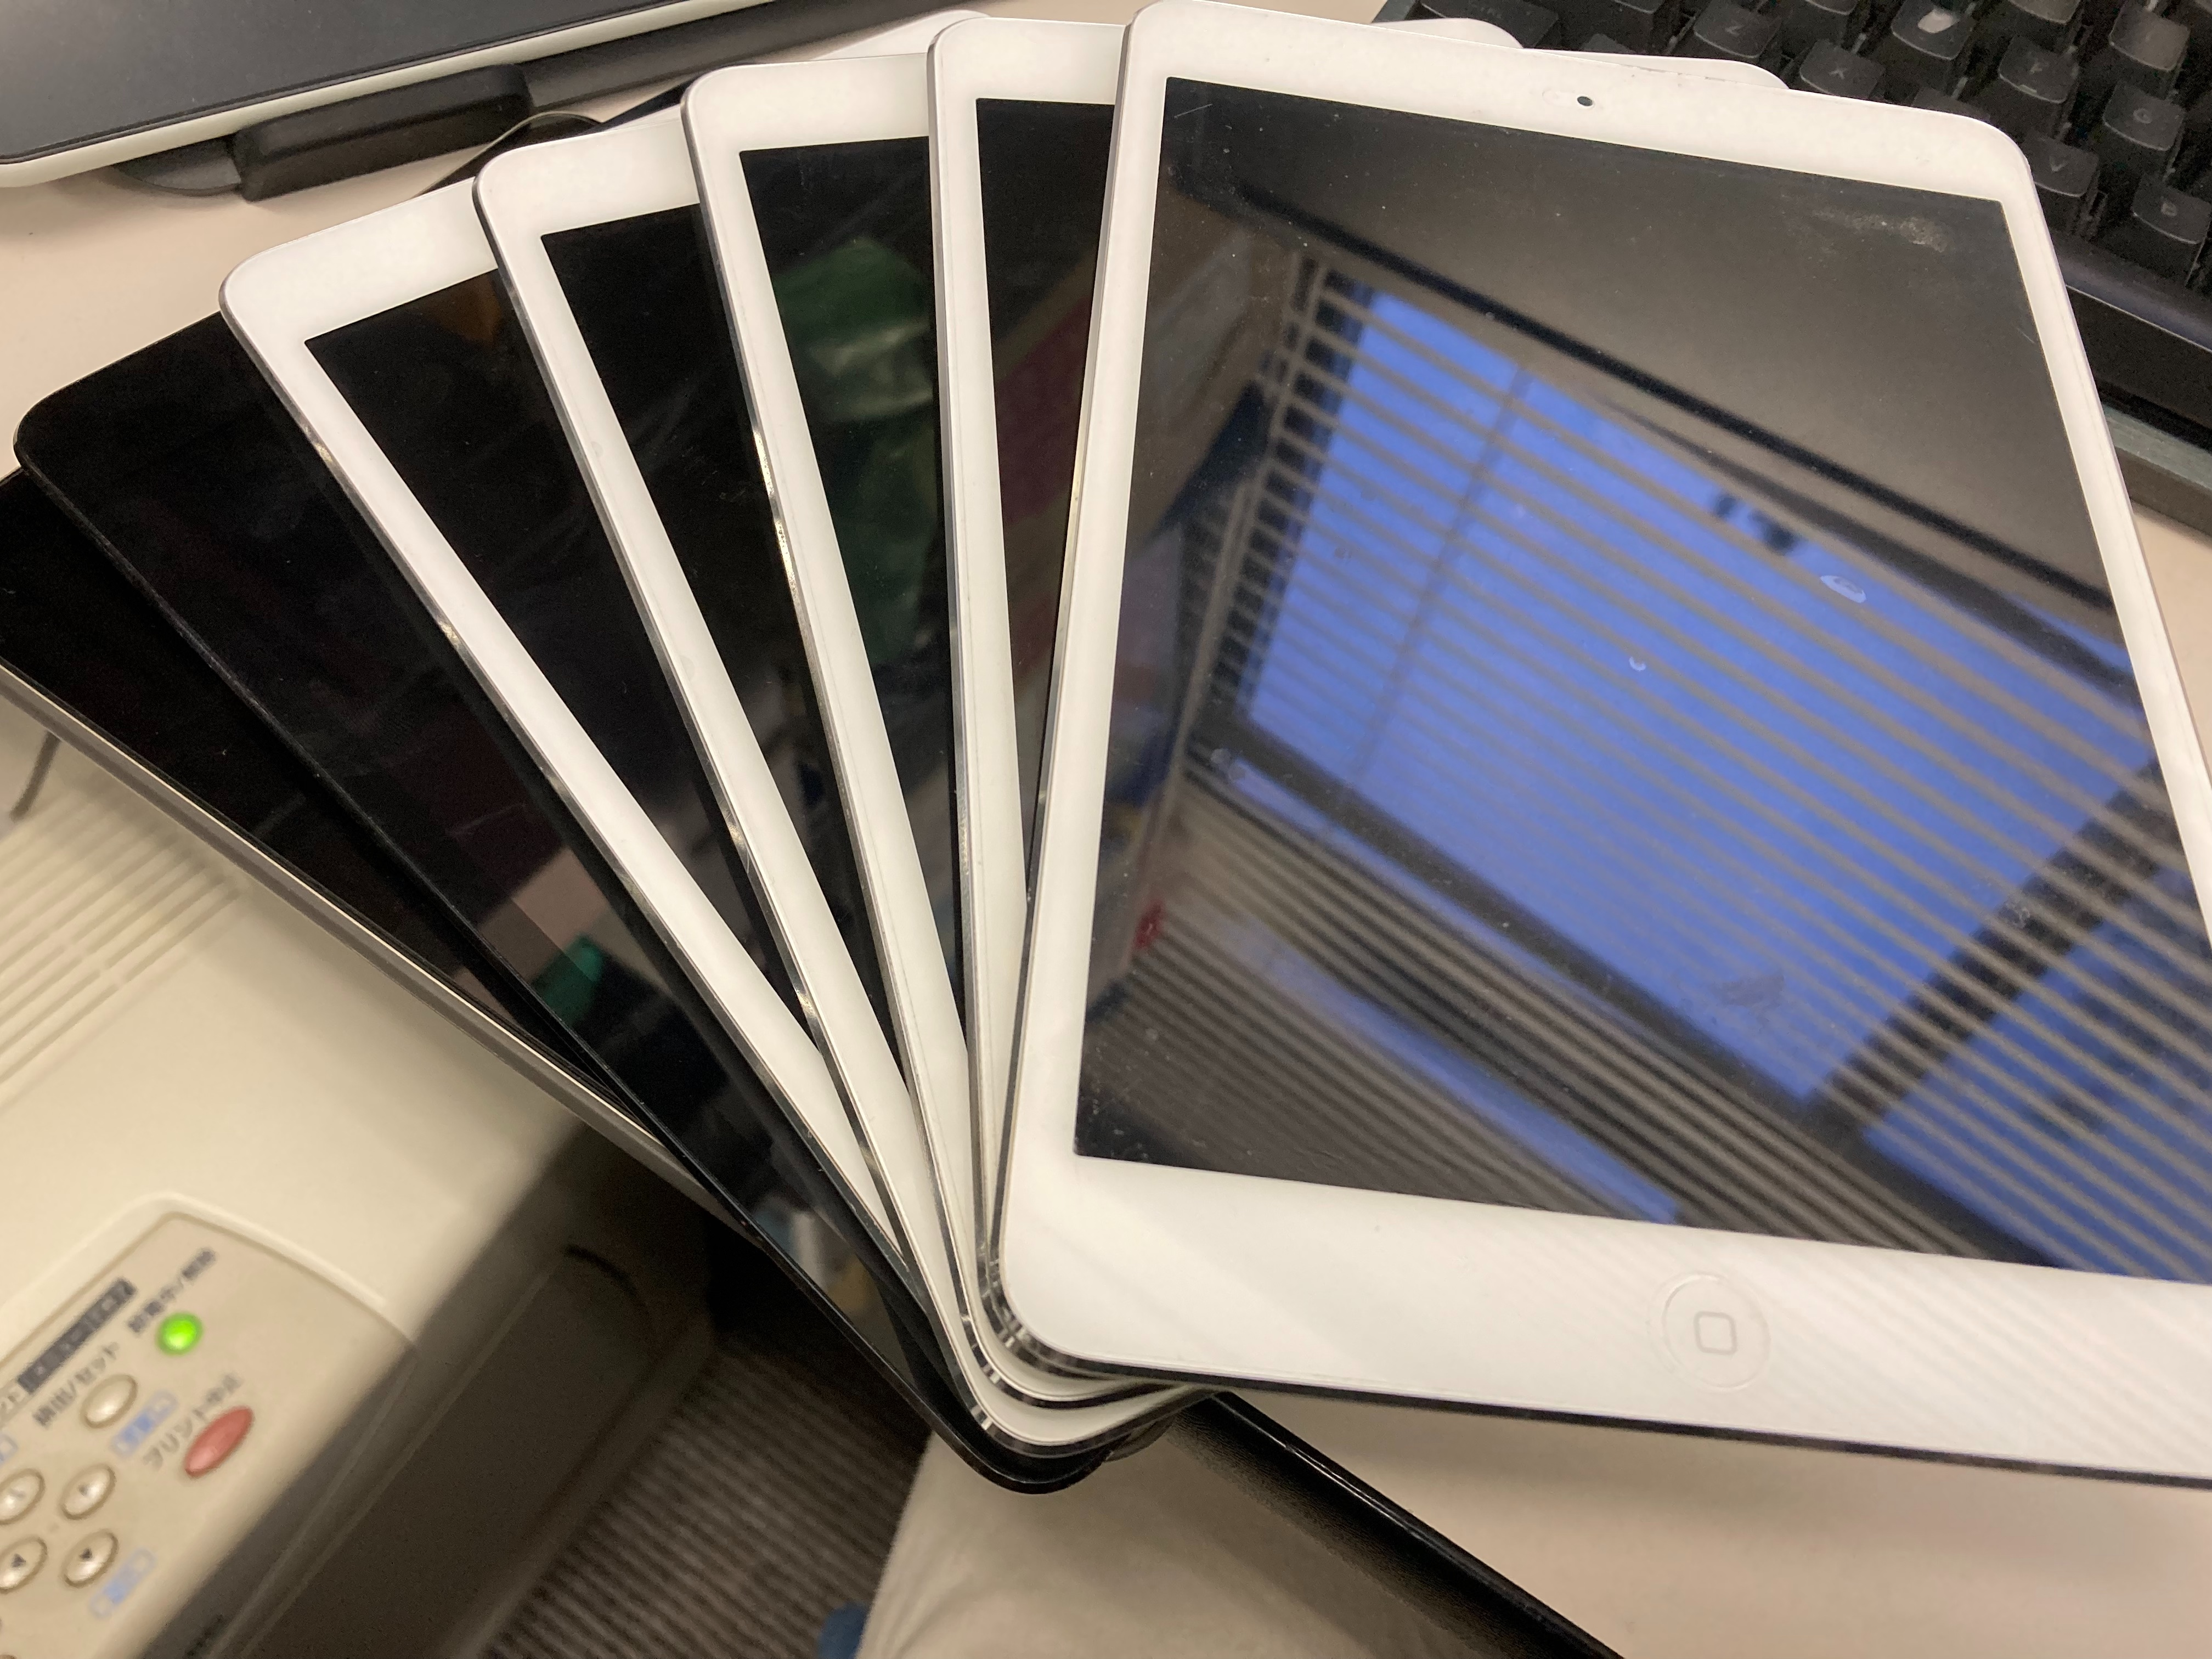
\includegraphics[width=\columnwidth]{./image/02-AboutSysken/iPad.jpg}
      \caption{タブレット端末}
    \end{minipage} &
    \hspace{0.04\columnwidth}
    \begin{minipage}[b]{0.40\columnwidth}
      \centering
      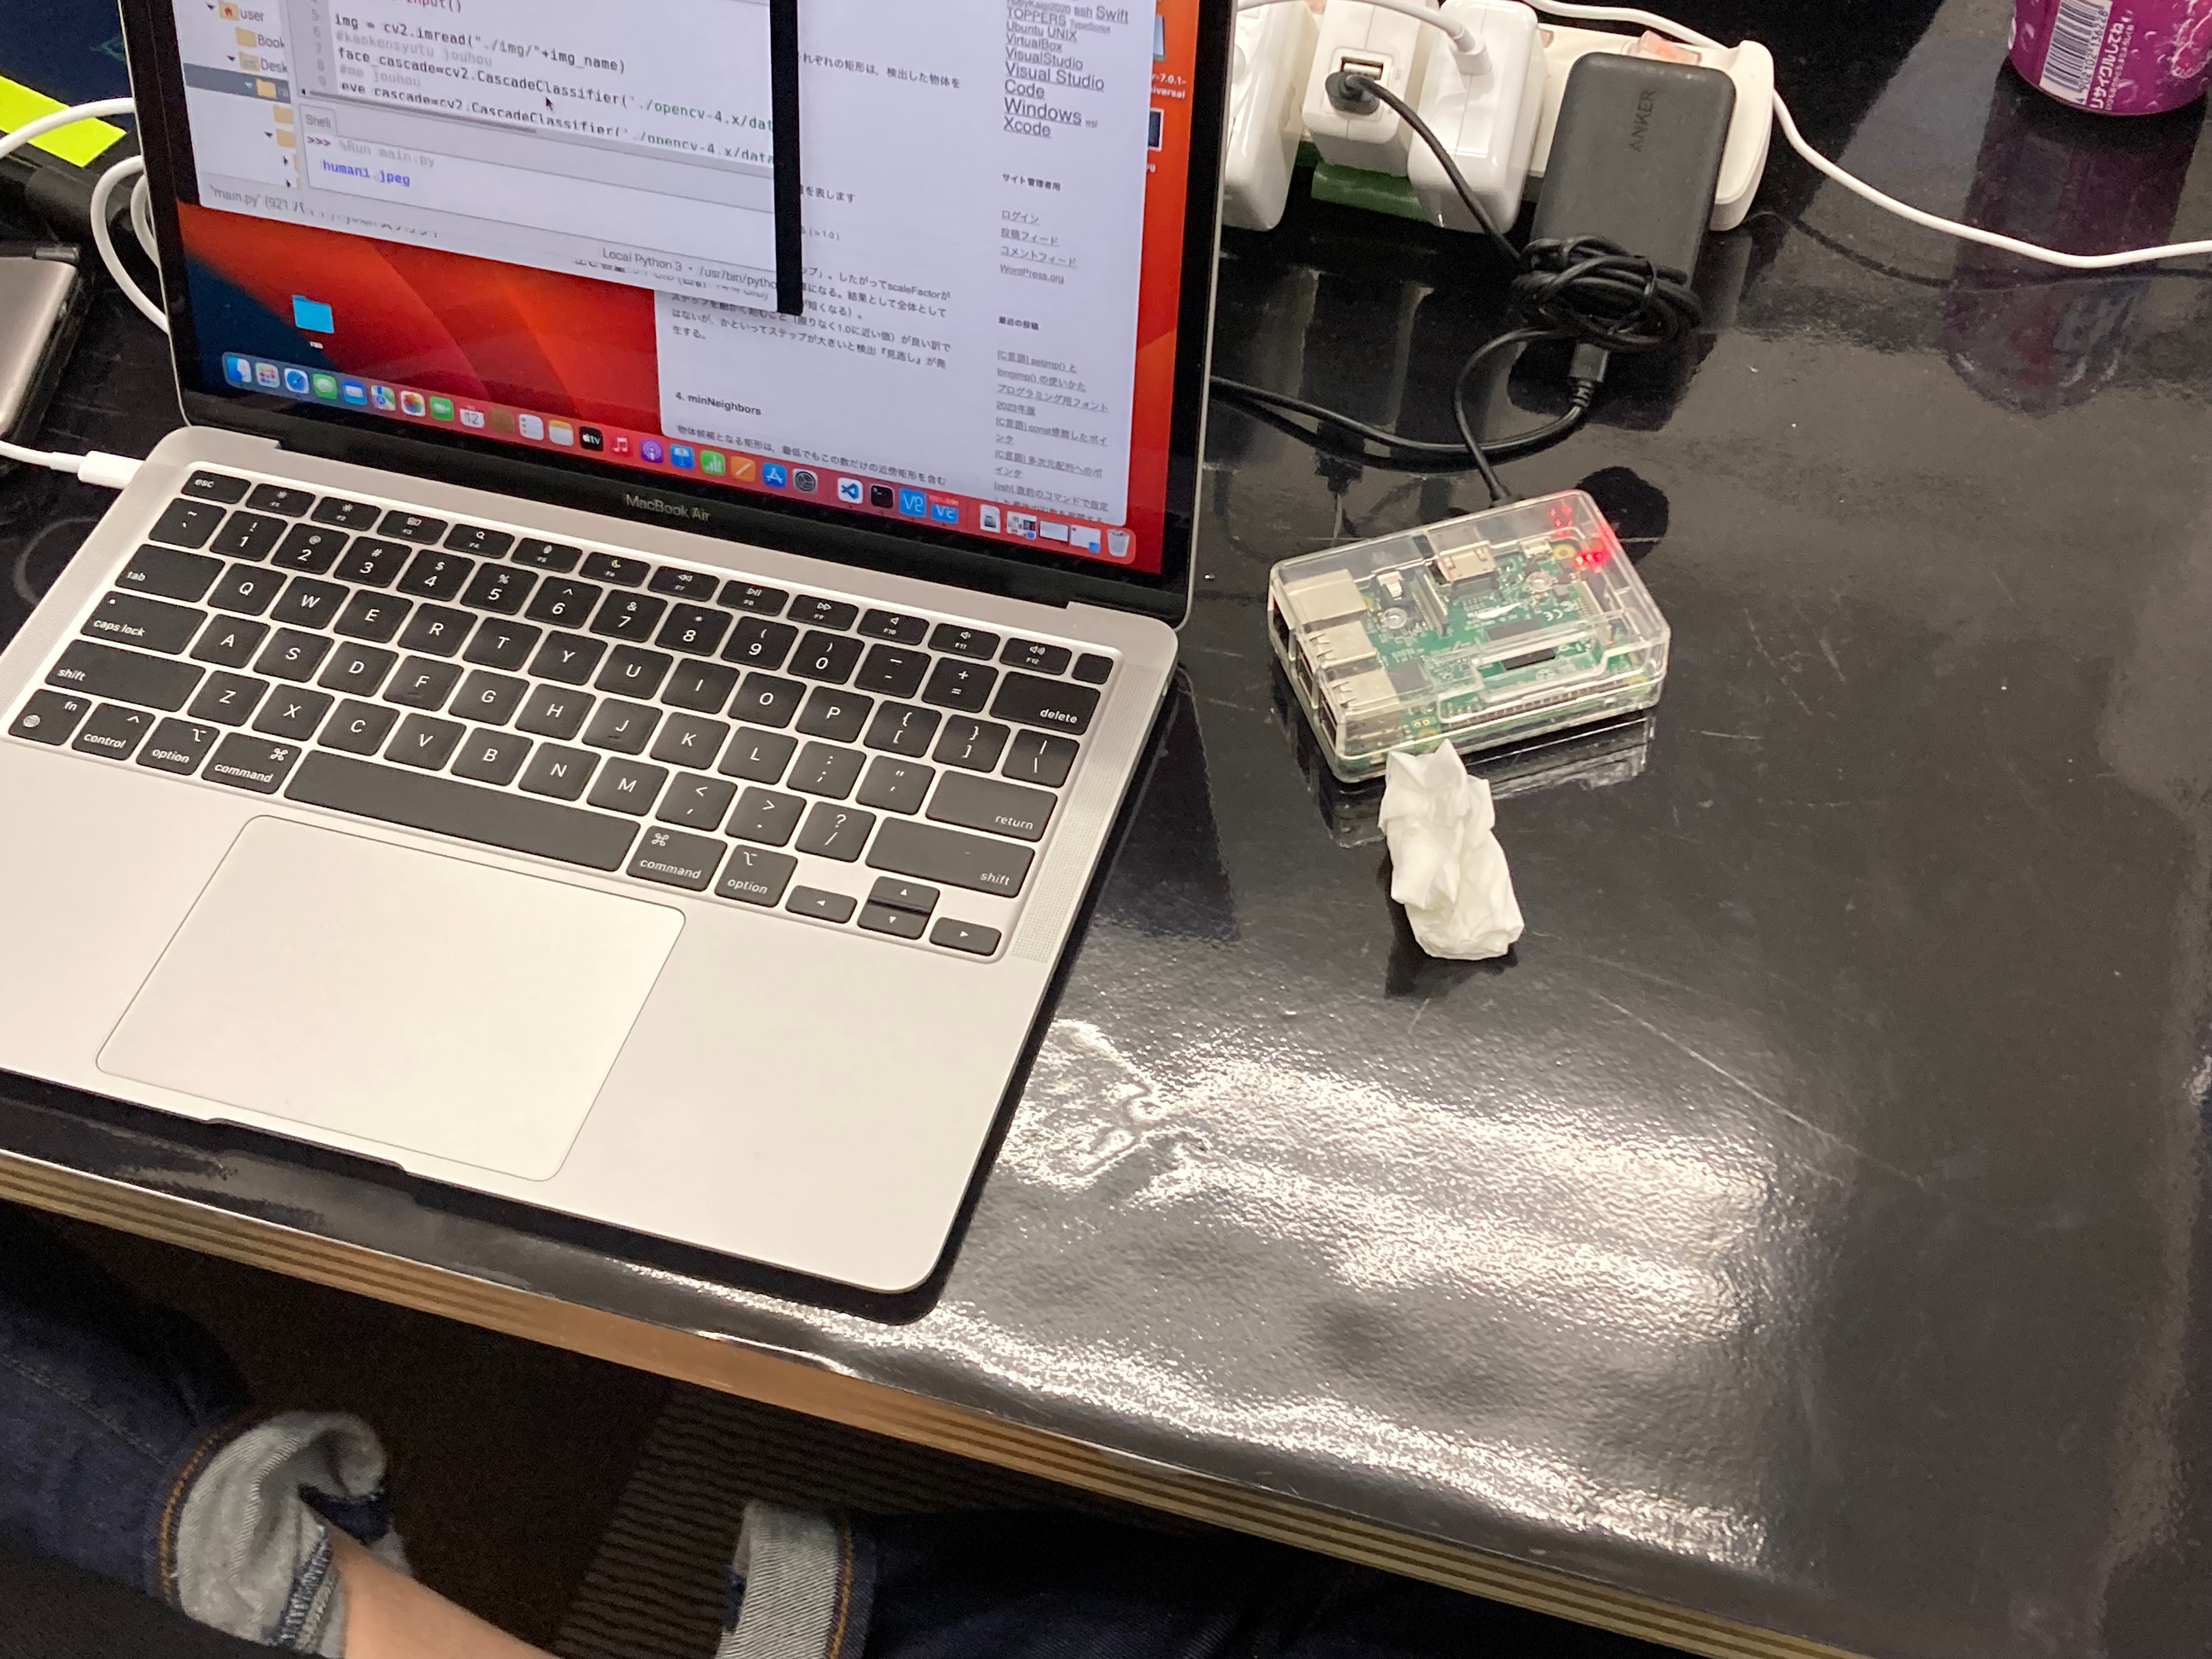
\includegraphics[width=\columnwidth]{./image/02-AboutSysken/RaspberryPi.jpg}
      \caption{Raspberry Pi}
    \end{minipage}
  \end{tabular}
\end{figure}

\section{この本について}
この本はシス研のメンバーが経験したこと、取り組んだことのアウトプットを目的としたものです。この本を通じて皆さんにはシス研のメンバーは具体的にどのような活動をしているのか知ってもらいたいと思います。 \\
また、シス研として本を出すのは今回が初めてなのでどうか温かい目で見ていただけると幸いです。

\section{まとめ}
ここまでお話をして来ましたが簡単にでもシス研について知ってもらうことはできたでしょうか?うまく伝えることができていたらとても嬉しいです。 \\
次のページからはメンバーの記事本編になります!シス研初めての本をよろしくお願いします!!